\documentclass[preprint, 3p,
authoryear]{elsarticle} %review=doublespace preprint=single 5p=2 column
%%% Begin My package additions %%%%%%%%%%%%%%%%%%%

\usepackage[hyphens]{url}

  \journal{Current Opinion in Environmental Science \&
Health} % Sets Journal name

\usepackage{graphicx}
%%%%%%%%%%%%%%%% end my additions to header

\usepackage[T1]{fontenc}
\usepackage{lmodern}
\usepackage{amssymb,amsmath}
% TODO: Currently lineno needs to be loaded after amsmath because of conflict
% https://github.com/latex-lineno/lineno/issues/5
\usepackage{lineno} % add
\usepackage{ifxetex,ifluatex}
\usepackage{fixltx2e} % provides \textsubscript
% use upquote if available, for straight quotes in verbatim environments
\IfFileExists{upquote.sty}{\usepackage{upquote}}{}
\ifnum 0\ifxetex 1\fi\ifluatex 1\fi=0 % if pdftex
  \usepackage[utf8]{inputenc}
\else % if luatex or xelatex
  \usepackage{fontspec}
  \ifxetex
    \usepackage{xltxtra,xunicode}
  \fi
  \defaultfontfeatures{Mapping=tex-text,Scale=MatchLowercase}
  \newcommand{\euro}{€}
\fi
% use microtype if available
\IfFileExists{microtype.sty}{\usepackage{microtype}}{}
\usepackage[]{natbib}
\bibliographystyle{elsarticle-harv}

\usepackage{graphicx}
\ifxetex
  \usepackage[setpagesize=false, % page size defined by xetex
              unicode=false, % unicode breaks when used with xetex
              xetex]{hyperref}
\else
  \usepackage[unicode=true]{hyperref}
\fi
\hypersetup{breaklinks=true,
            bookmarks=true,
            pdfauthor={},
            pdftitle={Biomonitoring of smoke exposure in firefighters: A review},
            colorlinks=false,
            urlcolor=blue,
            linkcolor=magenta,
            pdfborder={0 0 0}}

\setcounter{secnumdepth}{5}
% Pandoc toggle for numbering sections (defaults to be off)


% tightlist command for lists without linebreak
\providecommand{\tightlist}{%
  \setlength{\itemsep}{0pt}\setlength{\parskip}{0pt}}

% From pandoc table feature
\usepackage{longtable,booktabs,array}
\usepackage{calc} % for calculating minipage widths
% Correct order of tables after \paragraph or \subparagraph
\usepackage{etoolbox}
\makeatletter
\patchcmd\longtable{\par}{\if@noskipsec\mbox{}\fi\par}{}{}
\makeatother
% Allow footnotes in longtable head/foot
\IfFileExists{footnotehyper.sty}{\usepackage{footnotehyper}}{\usepackage{footnote}}
\makesavenoteenv{longtable}






\begin{document}


\begin{frontmatter}

  \title{Biomonitoring of smoke exposure in firefighters: A review}
    \author[Department of Chemistry and Chemical Biology]{Biban Gill%
  %
  }
  
    \author[Department of Chemistry and Chemical Biology]{Philip
Britz-McKibbin%
  \corref{cor1}%
  }
   \ead{britz@mcmaster.ca} 
      \affiliation[Department of Chemistry and Chemical Biology]{
    organization={McMaster University},addressline={1280 Main Street
West},city={Hamilton},postcode={L8S
4M1},state={Ontario},country={Canada},}
    \cortext[cor1]{Corresponding author}
  
  \begin{abstract}
  Biomonitoring of exposures to toxic contaminants from environmental
  smoke is important due to their deleterious impacts on human health,
  including cardiorespiratory diseases and cancer. This is particularly
  relevant for firefighters who are prone to extensive dermal exposure
  to smoke despite using personalized protective equipment. Reliable
  methods are needed for the analysis of sensitive yet specific
  biomarkers reflecting occupational smoke exposure, given various
  background sources. This review focuses on biomarkers used for
  measuring acute smoke exposure after fire suppression activities, such
  as biotransformed hydroxylated polycyclic aromatic hydrocarbons and
  their isomers in urine. Major challenges include developing optimal
  sampling approaches to capture transient smoke exposures, evaluating
  genetic and lifestyle contributions that modify risk assessment, as
  well as integrating clinically relevant biomarkers associated with
  oxidative stress, inflammation, and/or genotoxicity. Herein, we focus
  on robust biomarkers of recent smoke exposures and future perspectives
  aimed at implementing effective mitigation strategies for workplace
  protection of firefighters.
  \end{abstract}
    \begin{keyword}
    Smoke
exposures \sep Biomarkers \sep Biomonitoring \sep Firefighters \sep Polycyclic
aromatic hydrocarbons \sep Chromatography \sep 
    Mass spectrometry
  \end{keyword}
  
 \end{frontmatter}

\section{Introduction}\label{introduction}

Over half the global population is exposed to household smoke from the
burning of wood, coal, charcoal, or biomass for daily cooking and
heating needs \citep{1}. There is also an alarming exposure to
contaminants in particulate matter prevalent in rapidly expanding urban
settings of many developing countries. Together, environmental smoke
exposure from tobacco use and ambient air pollution is the fourth
leading risk factor for disease burden worldwide \citep{2}. However,
firefighters are at even greater risk for chronic exposure to smoke due
to their occupation, including a plethora of carcinogenic chemicals from
the combustion of wood and plastics \citep[\citet{4}, \citet{5}]{3}.
Occupational exposure to smoke increases the incidence of
cardiorespiratory illnesses (e.g.~chronic obstructive pulmonary disease,
cardiac infarction) and is associated with a higher risk for cancer in
firefighters \citep[\citet{7}]{6}. As a result, most states and
provinces across North America have introduced presumptive cancer
legislations providing firefighters with workers compensation for
job-related illnesses \citep{8}.

Biomonitoring of smoke exposure can be used as a tool to investigate
work protection factors to mitigate chronic disease risk and improve
long-term health outcomes for firefighters. Despite the use of personal
protective equipment during fire events, such as self-contained
breathing apparatuses to reduce inhalation exposure, higher cancer rates
are still prevalent among firefighters as compared with the general
public \citep{8}. Consequently, accurate assessment of the chemical
constituents in smoke is required to delineate multiple exposure
pathways that impact firefighters during training exercises and active
deployment, including initial fire suppression and subsequent overhaul
activities \citep[\citet{10}, \citet{11}]{9}. This includes hygienic
practices and personal protective equipment designed to reduce dermal
absorption of intoxicants because it remains the major route of exposure
for firefighters when inhalation is minimized \citep{12}.

Toxic substances identified in fire smoke include polycyclic aromatic
hydrocarbons (PAHs), volatile organic compounds (e.g.~methoxyphenols),
and asphyxiate gases (e.g.~carbon monoxide), in addition to various
other combustion-related contaminants (e.g.~dioxins) and inorganic
materials (e.g.~asbestos). As such, a growing number of smoke exposure
studies involving both structural/urban and wildland firefighters have
been reported \citep[\citet{13}, \citet{14}, \citet{15}, \citet{16},
\citet{17}]{6} since the International Agency for Research on Cancer
classified occupational exposure as a firefighter as possibly
carcinogenic to humans (Group 2B). Herein, we review the literature
since 2010 to examine best practices for assessing smoke exposure in
firefighters that is also relevant to other occupations
(e.g.~asphalt/coke oven workers), including biomarkers applicable to
risk assessment using validated instrumental protocols for their
quantitative determination.

\section{Biomarkers of smoke
exposure}\label{biomarkers-of-smoke-exposure}

For a biomarker to be considered an effective indicator of smoke
exposure, it must demonstrate adequate sensitivity, specificity, and
robustness for its routine analysis given numerous background sources
from diet and lifestyle, such as intake of charred/smoked meats, and
tobacco smoking that may not be accurately captured by self-reported
questionnaires \citep{18}. To date, several compounds identified in
human biofluids have been proposed as putative biomarkers of wood smoke
exposure in firefighters including carboxyhemoglobin, PAH metabolites,
PAH--DNA adducts, methoxyphenols (MPs), and levoglucosan \citep{19}.

Carbon monoxide is a major contributor to acute toxicity from smoke
inhalation owing to the formation of elevated levels of
carboxyhemoglobin in blood that impairs oxygen transport to vital organs
\citep{20}. However, an association with smoke exposures and circulating
carboxyhemoglobin was only reported to be significant in wildland
firefighters when carbon monoxide levels exceeded 5 ppm \citep{19}.
Carboxyhemoglobin thus demonstrates poor sensitivity when evaluating
subacute intoxification, and it does not allow for assessment of
exposure to carcinogens in firefighters \citep{21}. In addition,
sampling of blood is invasive, while alveolar breath for carbon monoxide
assessment is impractical to collect from firefighters during emergency
fire events \citep{22} unlike wearable devices that enable real-time
monitoring of heart rate, body temperature, and/or oxygen saturation
\citep{23}.

PAHs are largely generated as a result of incomplete combustion of
organic material via a hydrogen abstraction acetylene addition mechanism
\citep{24}. With more than 100 different species characterized in
complex smoke mixtures, 16 PAHs have been classified as possible
carcinogens and priority pollutants \citep{25}. Exposure to PAHs is
likely the primary cause for the high cancer rates in firefighters
because of the bioactivation of these compounds into reactive
intermediates that form covalent adducts to DNA \citep{26}. PAHs can be
measured directly on skin (i.e.~dermal deposition via skin wipes), as
well as in blood and urine; however, their short half-lives in
circulation make it difficult to analyze PAHs after a transient exposure
event. In contrast, analysis of biotransformed hydroxylated PAH
metabolites (OH-PAHs) in urine is far more practical for assessment of
recent smoke exposures within about 24 h \citep[\citet{27}]{19}. OH-PAHs
are metabolized in the liver and excreted in urine predominately as
their glucuronide conjugates. However, PAHs having more than four carbon
rings, including the more toxic benzo {[}a{]}pyrene (BaP), are
eliminated primarily in the feces \citep{28}, and thus, their urinary
OH-PAH concentrations are often below detection thresholds \citep{12}
even after offline sample preconcentration of large urine volumes
(\textgreater5 mL) by solid-phase extraction.

Several studies have evaluated smoke exposure based on reporting the sum
total or absolute concentrations of specific OH-PAH metabolites in urine
after normalization to creatinine to correct for differences in
hydration status when relying on single-spot urine specimens (Table 1).
Frequently measured urinary OH-PAH metabolites include 1-hydroxypyrene
(OH-Pyr), as well as various isomers of hydroxynapthalene (OH-Nap),
hydroxyphenathrene (OH-Phe), and hydroxyfluorene (OH-Flu) after their
enzymatic deconjugation. For instance, Keir et al. \citep{29} reported a
significant elevation in mean urinary OH-PAH concentrations ranging from
2.9- to 5.3-fold, 18 h after on-shift firefighting events as compared
with matching pre-exposure baseline, office workers at fire stations,
and nonsmoking healthy controls as shown in Figure 1. Furthermore, there
was a 4.3-fold average increase in urinary mutagenicity reported in
postfire suppression event urine samples collected from active duty
firefighters; however, no changes in urinary indicators of lung injury
and inflammation were reported.

\begin{longtable}[]{@{}
  >{\raggedright\arraybackslash}p{(\columnwidth - 8\tabcolsep) * \real{0.1588}}
  >{\raggedright\arraybackslash}p{(\columnwidth - 8\tabcolsep) * \real{0.1186}}
  >{\raggedright\arraybackslash}p{(\columnwidth - 8\tabcolsep) * \real{0.1715}}
  >{\raggedright\arraybackslash}p{(\columnwidth - 8\tabcolsep) * \real{0.5091}}
  >{\raggedright\arraybackslash}p{(\columnwidth - 8\tabcolsep) * \real{0.0420}}@{}}
\toprule\noalign{}
\begin{minipage}[b]{\linewidth}\raggedright
Urinary OH-PAHs
\end{minipage} & \begin{minipage}[b]{\linewidth}\raggedright
Study cohort
\end{minipage} & \begin{minipage}[b]{\linewidth}\raggedright
Method/sample workup
\end{minipage} & \begin{minipage}[b]{\linewidth}\raggedright
Major findings
\end{minipage} & \begin{minipage}[b]{\linewidth}\raggedright
Reference
\end{minipage} \\
\midrule\noalign{}
\endhead
\bottomrule\noalign{}
\endlastfoot
OH-Pyr, 1-OH-Nap, 2-OH-Flu, OH-Phe, 3-OH-B{[}a{]}P, 1-OH-Ace &
Structural firefighters (n~=~96 nonexposed; 57 exposed) & LC-FLD
(solid-phase extraction of 10 mL of urine) & Median levels of total
OH-PAHs reported as 1.7- to 35-fold higher exposure than in nonexposed
controls. OH-Pyr was the least abundant one of the 6 urinary OH-PAHs. &
Oliveira et~al.~(2016) \\
OH-Pyr, 1-OH-Nap, 2-OH-Flu, OH-Phe, 3-OH-B{[}a{]}P, 1-OH-Ace &
Structural firefighters (8 fire stations) & LC-FLD (solid-phase
extraction of 10~mL of urine) & Positive correlations reported between
ambient PAHs and urinary OH-PAHs for firefighters at 4 of 8 fire
stations. Postshift urinary OH-Pyr levels were below that suggested by
the American Conference of Government Industrial Hygienists. & Oliveira
et~al.~(2017) \\
OH-Pyr, 1-OH-Nap, 2-OH-Flu, OH-Phe, 3-OH-B{[}a{]}P, 1-OH-Ace & Wildland
firefighters (n~=~108) & LC-FLD (solid-phase extraction of 10~mL of
urine) & Total OH-PAHs increased by 76â€``412\% after regular tobacco
consumption. Fire combat resulted in increases of 158â€``551\%. 2-OH-Flu
was most affected by fire combat, while 1-OH-Nap and 1-OH-Ace were most
pronounced in tobacco smokers. & Oliveira et~al.~(2017) \\
OH-Pyr, 1-OH-Nap, 2-OH-Flu, OH-Phe, 3-OH-B{[}a{]}P, 1-OH-Ace &
Structural firefighters (n~=~15 nonexposed; 18 exposed) & LC-FLD
(solid-phase extraction of 10~mL of urine) & Total OH-PAHs were
1.96-fold higher in exposed firefighters, with 1-OH-Nap and 1-OH-Ace
being the most abundant smoke biomarkers. DNA damage and oxidative
stress were also elevated in exposed firefighters. & Oliveira
et~al.~(2018) \\
OH-Pyr, 1-OH-Nap, 2-OH-Nap, 2-OH-Flu, 3-OH-Flu, 1-OH-Phe, 2-OH-Phe,
3-OH-Phe, 4-OH-Phe & Wildland firefighters (n~=~14) & LC-MS/MS (on-line
solid-phase extraction with 0.2~mL of urine) & Preshift median
concentrations of OH-PAHs were higher than median concentrations
reported for US population, with the exception of 1-OH-Nap, whereas
4-OH-Phe concentrations were associated with levoglucosan. & Adetona
et~al.~(2017) \\
OH-Pyr & Wildland firefighters (n~=~12) & LC-FLD (solid-phase extraction
of 10~mL of urine) & No significant difference reported in urinary
mutagenicity between firefighters on burn days vs nonburn days, but a
significant correlation was observed between urinary mutagenicity and
urinary OH-Pyr. & Adetona et~al.~(2019) \\
OH-Pyr, OH-Nap, OH-Flu, OH-Phe & Structural firefighters (n~=~15) &
ELISA & Median concentrations for all OH-PAHs increased in urine from
before to after 3Â~h of training exercises. A 30-fold increase in OH-Pyr
was reported with the highest levels in oriented strand board fire
exercises. & Fent et~al.~(2019) \\
OH-Pyr, OH-Phe, OH-Flu, OH-Nap & Structural firefighters (n~=~34) &
LC-MS/MS (on-line solid-phase extraction with 0.1~mL of urine) & Median
concentrations for all OH-PAHs increased in urine from before to after
3Â~h of training exercises. A 30-fold increase in OH-Pyr was observed
with the highest levels observed in oriented strand board fire
exercises. & Fent et~al.~(2014) \\
OH-Pyr, 2-OH-Nap, 1-OH-Phe, 3-OH-Phe, 2-OH-Flu 9-OH-Flu & Wildland
firefighters (n~=~42) & LC-MS/MS (dilution and direct injection);
GC-HRMS (solid-phase extraction and derivatization) & Good mutual
agreement between LC-MS/MS and GC-HRMS for OH-Pyr that was dependent on
enzyme hydrolysis reaction times. 3-OH-Phe and 9-OH-Flu were positively
correlated with OH-Pyr, with urinary OH-Pyr levels below the recommended
biological exposure index. & Gill et~al.~(2019) \\
OH-Pyr & Wildland firefighters (n~=~42) & LC-MS/MS (dilution and direct
injection) & OH-Pyr was detected in 71\% of firefighter urine samples
after deployment. Among the samples collected within 48Â~h, OH-Pyr was
correlated with estimated exposure. Lower urinary OH-Pyr was reported in
firefighters with a high skin exposure mitigation index. & Cherry
et~al.~(2019) \\
OH-Pyr, OH-Nap & Structural firefighters (n~=~16) & LC-FLD (solid-phase
extraction); GC-ECD (derivatization) & Highest excretion of OH-Pyr was
reported when burning conifer plywood and chipboard, while the lowest
was pine and sprucewood, indicating burning material impacts smoke
exposure. & Laitinen et~al.~(2010) \\
OH-Pyr, OH-Nap & Structural firefighters (n~=~13) & LC-FLD (solid-phase
extraction); GC-ECD (derivatization) & Dermal exposure of PAHs delays
excretion of OH-Pyr and OH-Nap. Biological action limit values for
1-OH-Pyr were reported as 53Â~nM. & Laitinen et~al.~(2012) \\
OH-Pyr, 1-OH-Nap, 2-OH-Nap, 2-OH-Flu, 9-OH-Flu, 3-OH-Flu, 3-OH-Phe,
4-OH-Phe, 2-OH-Phe & Structural firefighters (n~=~28) & GC-MS/MS
(solid-phase extraction and derivatization) & A suite of MPs and urinary
OH-PAH metabolites were sensitive smoke biomarkers in urine samples
24Â~h after exposure, with operational roles of firefighters in burn
houses being a large contributor to variations. & Fernando
et~al.~(2016) \\
OH-Pyr & Structural firefighters (n~=~22) & LC-FLD (solid-phase
extraction) & Skin deposition of pyrene and urinary OH-Pyr did not
differ before and after work shifts, irrespective of fire extinguishing
role. Increased work shift was not associated with genotoxicity based on
oxidative damage to DNA. & Andersen et~al.~(2018) \\
OH-Pyr, OH-Nap, OH-Flu, OH-Phe, & Structural firefighters (n~=~27
firefighters; 18 office workers) & GC-MS/MS (liquid-liquid extraction
and derivatization) & A significant 2.9- to 5.3-fold increase in average
postevent urinary PAH metabolites was observed, with 54\% of the
variation in fold changes being due to air vs.~skin exposure. Postevent
urinary mutagenicity showed a significant increase by 4.3-fold for
postshift urine samples. & Keir et~al.~(2017) \\
OH-Pyr, & Wildland firefighters (n~=~22) & LC-FLD & Particulate matter
measurements indicated the use of personal protective equipment
effectively prevented inhalation exposure, but exposure still occurred
owing to early removal of equipment. Skin deposition of pyrene was
correlated to urinary OH-Pyr for most firefighters. & Wingfors
et~al.~(2017) \\
\end{longtable}

\begin{figure}
\centering
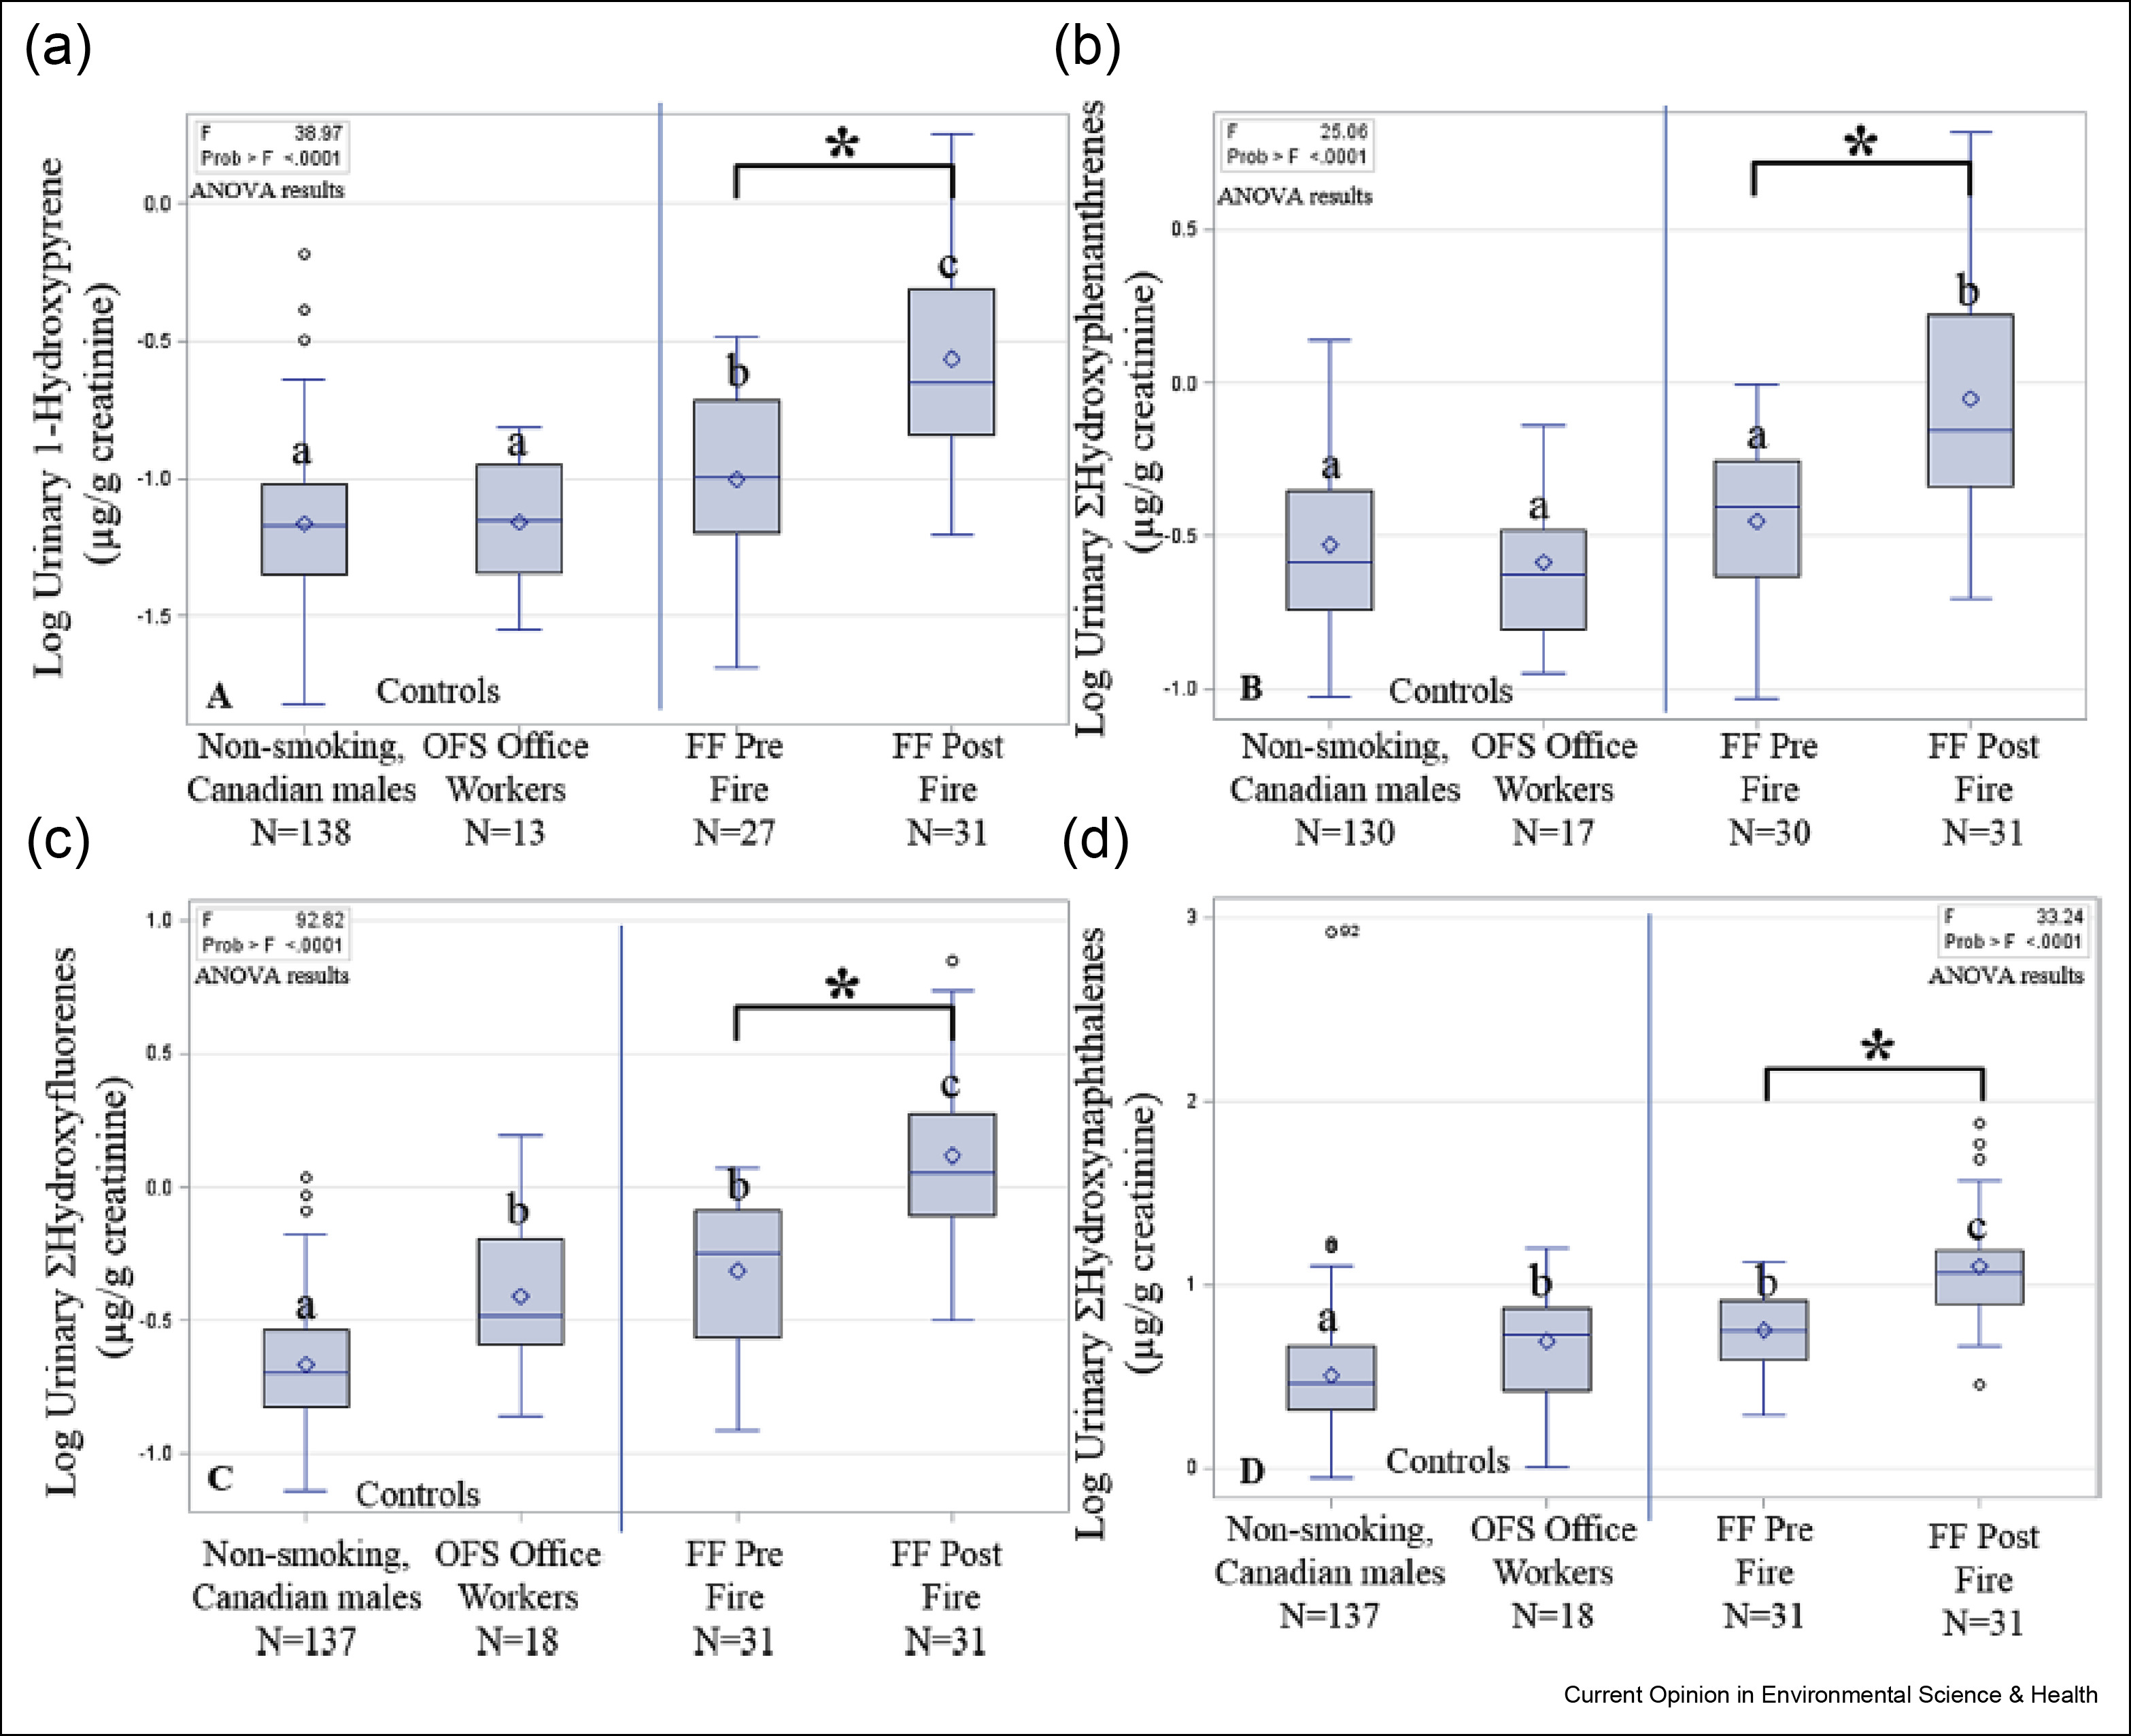
\includegraphics{./Figures/Figure1.jpg}
\caption{An increase in OH-PAH concentrations (as indicated by the
single asterisks, p \textless{} 0.0001) in urine collected in
firefighters 18 h after exposure as compared with their baseline levels
when using GC--MS/MS as reported by Keir et al. \citep{29}. Box-whisker
plots for urinary (a) 1-hydroxypyrene, as well as total isomers for (b)
hydroxyphenanthrene, (c) hydroxyfluorene, and (d) hydroxynapthalene are
shown for firefighters both before and after fire events as compared
with a cohort of nonsmoking Canadian males, and nondeployed office
workers at the fire station as controls {[}29{]}. The box limits
represent the interquartile range (i.e.~25th to 75th percentile), the
line and diamond are the median and mean concentration, respectively;
the whiskers extent to the 5th and 95th percentiles, and circles are
outliers. ANOVA, analysis of variance; FF, firefighter; GC, gas
chromatography; MS/MS, tandem mass spectrometry; OH-PAH, hydroxylated
polycyclic aromatic hydrocarbons. Adapted from the study by Keir et
al.~(2017) with permission from ACS publications.}
\end{figure}

Fernando et al. \citep{3} analyzed a suite of OH-PAHs and other
combustion by-products of wood smoke that were elevated in 24-h
postexposure urine samples collected in firefighters after training
exercises in burn houses. Smoke exposures were dependent on the specific
operational role of firefighters, as well as other variables in the five
different sites tested, such as burn house dimensions, fire intensity,
and local hygienic practices involving cleaning of their bunker gear and
self-contained breathing apparatus. Similarly, Oliviera et al.
\citep{14} measured elevated concentrations of six urinary OH-PAHs in
wildland firefighters at 1.7- to 35-fold higher than in nonexposed
participants, highlighting a large variability in smoke exposures.
Although there are numerous PAH metabolites excreted in the urine,
OH-Pyr is most widely used for biomonitoring of smoke exposure. Urinary
OH-Pyr is widely used for biomonitoring of recent smoke exposures due to
the natural abundance of pyrene in most smoke mixtures, which is also
excreted in urine as a single isomer with a half-life ranging from 6 to
32 h depending on the exact exposure pathway \citep[\citet{30}]{27}.
Ciarrocca et al. \citep{31} performed a meta-analysis study to confirm
the validity of urinary OH-Pyr as a biomarker of occupational exposure
to PAHs provided that other environmental, genetic, and lifestyle
factors are considered. Recently, Wingfors et al. \citep{12} reported
that among 8 urinary PAH metabolites analyzed in their study, OH-Pyr was
the most useful indicator of transient smoke exposure with elevated
urinary concentrations measured at 6 and 20 h after exposure, which also
had the strongest correlation to particle-bound PAH dermal exposure
unlike other urinary OH-PAH metabolites as shown in Figure 2. However,
there were some exceptions to this linear model likely reflecting other
routes of exposure among certain firefighters participating in this
study \citep{12}. Indeed, delays to urine collection from wildland
firefighters contribute to a significant underestimate of their true
exposures in the field \citep[\citet{32}]{30} that is well below the
recommended occupational exposure limit for urinary OH-Pyr of 1.0
umol/mol creatinine \citep{33} or 0.5 umol/mol creatinine as recommended
by the American Conference of Government Industrial Hygienists.

\begin{figure}
\centering
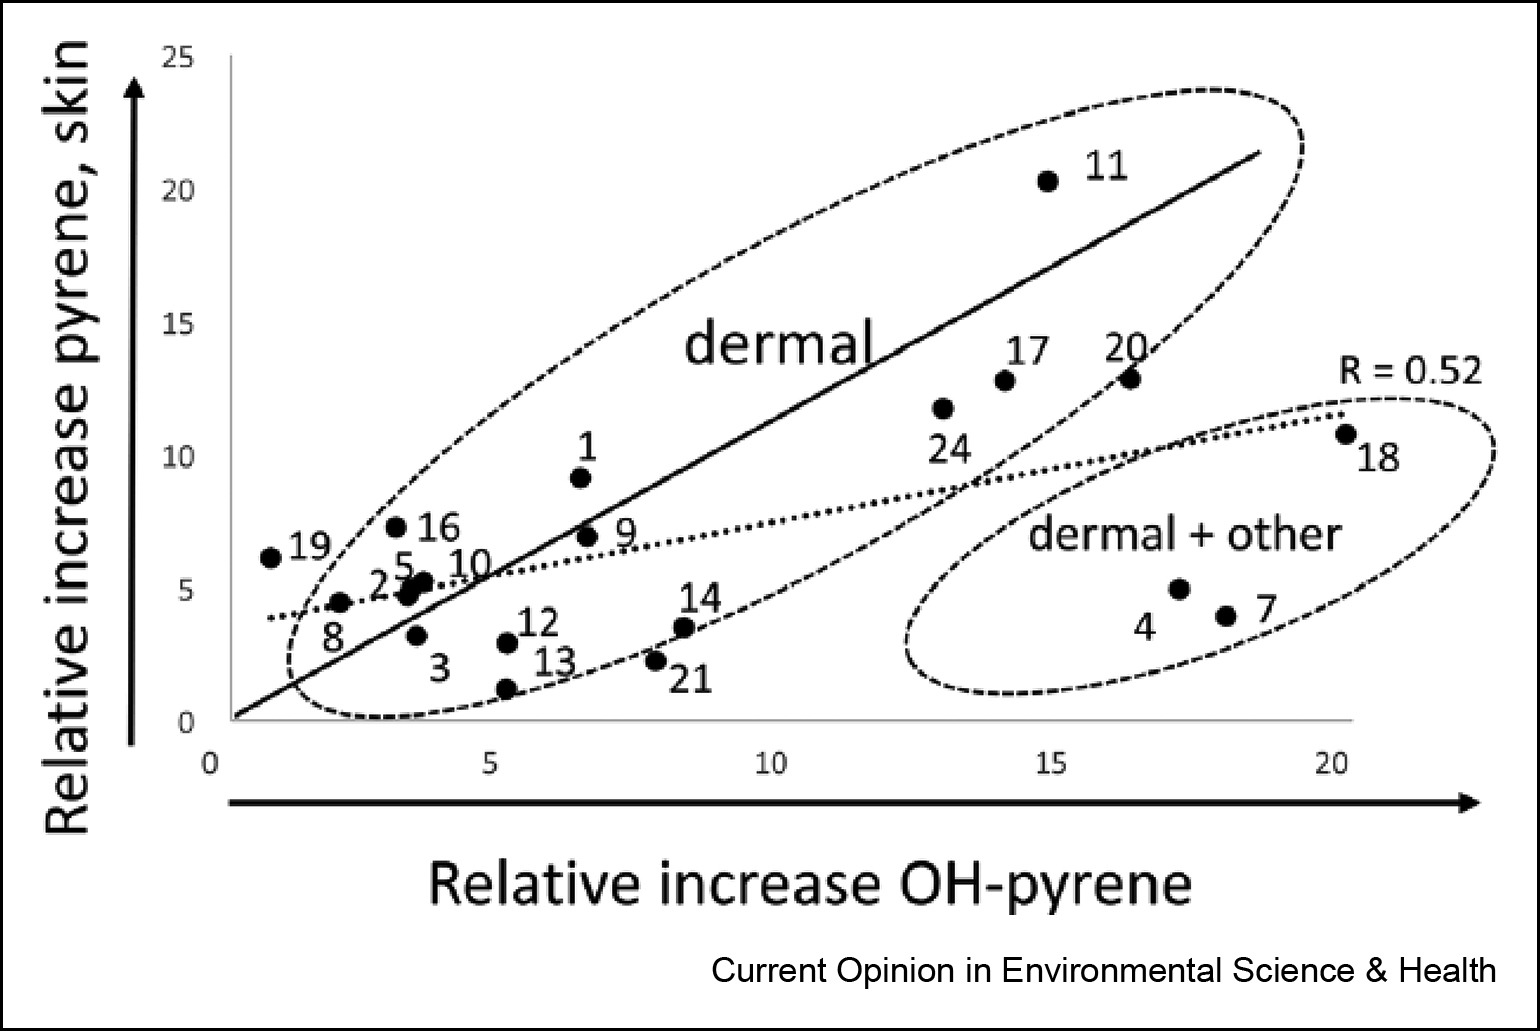
\includegraphics{./Figures/Figure2.jpg}
\caption{A positive correlation between urinary OH-Pyr collected at 6 h
after exposure and pyrene deposited on the neck of volunteer
firefighters as reported by Wingfors et al. \citep{12}. This study
indicated a predominant dermal exposure route for nonsmoking
firefighters who were equipped with a self-contained breathing
apparatus. However, three participants deviated from this linear model,
which was likely due to underlying differences in their metabolism
and/or other exposure routes. OH-Pyr, 1-hydroxypyrene. Reprinted from
the study by Wingfors et al.~(2018) with permission from Oxford
Academic.}
\end{figure}

The most widely used instrumental methods for PAH and OH-PAH analysis
include gas chromatography (GC) with tandem mass spectrometry (MS/MS)
and increasingly high resolution MS (HRMS) that is optimal for
nontargeted screening of chemical exposures in the environment
\citep{34}. In addition, liquid chromatography (LC) coupled to either
fluorescence detection (FLD) and MS/MS allows for direct analysis of
OH-PAHs and their intact glucuronides without complicated and
time-consuming sample workup procedures, such as enzymatic hydrolysis
and chemical derivatization. Nevertheless, extensive sample cleanup is
still needed to reduce background interferences while lowering detection
limits when using immunoaffinity, liquid extraction or solid-phase
extraction protocols. Table 1 summarizes recent smoke exposure studies
involving the analysis of urinary OH-PAHs from firefighters that also
outline different analytical methods, study designs, and major outcomes.
Recently, Gill et al. \citep{30} performed an interlaboratory method
comparison between LC-MS/MS and GC-HRMS for urinary OH-Pyr determination
from firefighters deployed in the 2016 Fort McMurray wildfire. The study
revealed a modest bias of 39\% when comparing both methods, which was
mainly due to incomplete deconjugation of OH-Pyr in the LC-MS/MS
protocol based on enzymatic reaction conditions recommended by the
reagent supplier \citep{30}. Consequently, standardized operating
protocols are critical for reliable urinary OH-Pyr determination that is
also dependent on the specific enzyme source and its glucuronidase
and/or sulfatase activity that can vary between batches. In addition,
enzyme impurities may contribute to unanticipated substrate degradation
and oxidation artifacts resulting in method bias \citep{35}.

PAH--DNA adducts have also been used as more biologically relevant
indicators of intoxification and PAH-initiated carcinogenesis from
chronic smoke exposures in firefighters. They also show promise as
dose-response measures that better reflect the impact of exposure,
absorption, distribution, and metabolism of harmful chemical
constituents from smoke. For example, bioactivation of PAHs by specific
cytochrome P450 isoforms result in the formation of DNA adducts to
adenine and guanine bases via PAH diol epoxides within cells/tissue,
such as BaP-DNA adducts in lymphocytes \citep{19}. Pratt et al.
\citep{36} used immunohistochemistry to localize PAH--DNA adducts from
human tissue biopsies for semiquantitative assessment of the impact of
PAH exposures. However, reliance on tissue biopsies is a limiting factor
for this approach, given the need for invasive sample collection, which
is impractical for routine biomonitoring of firefighters after emergency
fire suppression events. As a result, leukocytes have been used as more
accessible circulating white blood cells from whole blood for DNA
extraction with BPDE--DNA adducts analyzed by commercial immunoassay
kits. However, there were no significant differences in PAH--DNA adducts
formation in leukocytes measured between before and after shift samples
in a study involving volunteer firefighters \citep{37}, thus making this
a less sensitive biomarker for evaluating transient smoke exposures.
Alternatively, biomarkers of oxidative DNA damage are more readily
measured in urine by LC-MS/MS (e.g.~8-hydroxydeoxyguanosine), which can
be correlated to biotransformed PAH carcinogens, such as the glucuronide
and sulfate conjugates of 3-OH-BaP \citep{38}.

MPs in wood smoke are formed as a result of lignin combustion, which
makes up 18--35\% of wood by mass. Studies have suggested their use as
potential biomarkers of smoke exposure as they are readily detectable in
urine \citep{19}. Fernando et al. \citep{3} reported that MPs are on
average 5--10 times higher in concentration than the most abundant PAHs
in smoke, such as naphthalene and phenanthrene. Several MP analogues
were significantly elevated in firefighters in postexposure urine
samples similar to trends measured for OH-PAHs; however, little is known
about their toxicity in humans although animal studies indicate their
potential for impaired lung function. However, some MPs (e.g.~vanillin,
eugenol) are not reliable smoke biomarkers, given their ubiquitous use
in various foods and flavorants. In contrast, other MPs
(e.g.~methylsyringol, propylsyringol) are more specific indicators of
recent wood smoke exposure with an optimal detection window in urine
within 2--6 h \citep{19} similar to 2-OH-Nap \citep{39}. Importantly,
`whole-body' dermal exposure was evident in firefighters after training
exercises in burn houses when measuring the total amount of MPs and PAHs
from skin wipes sampled at five different body locations after exposure
as shown in Figure 3. This work highlights that current personal
protective equipment for firefighters are not designed to prevent skin
absorption of chemical constituents from smoke. Greater exposures have
also been reported among firefighters not wearing their flash hood
equipment during on-shift fire suppression activities \citep{29}, and
poor skin hygiene practices exacerbated by prolonged emergency
deployment \citep{32}.

\begin{figure}
\centering
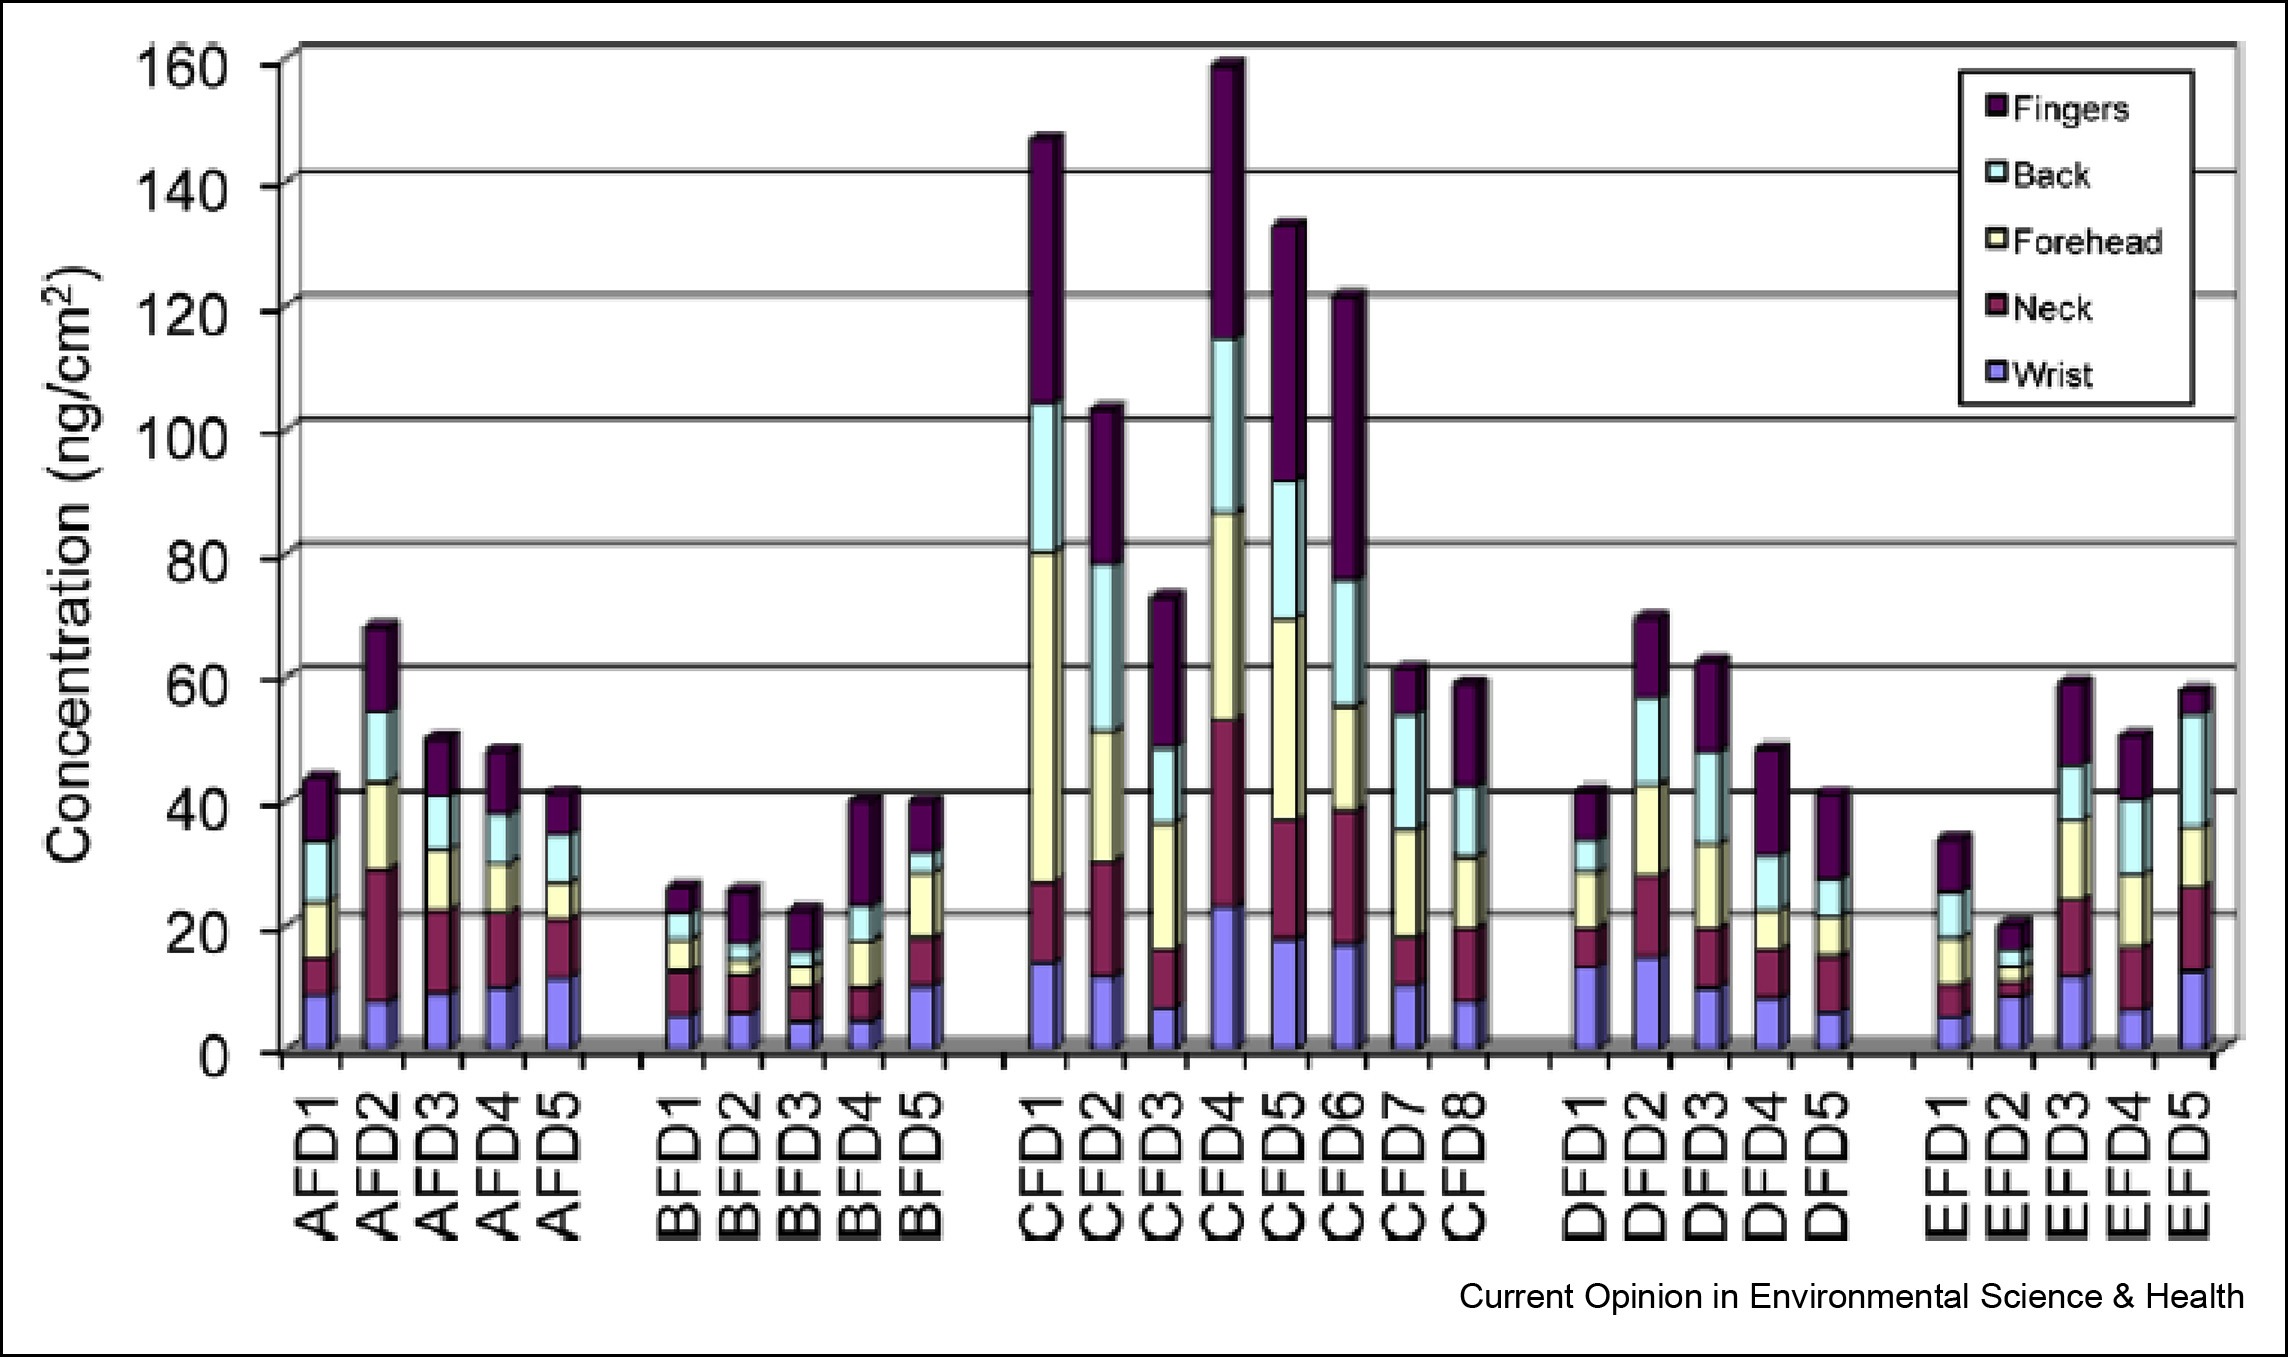
\includegraphics{./Figures/Figure3.jpg}
\caption{Whole-body dermal exposure demonstrated by the collection of
skin wipes from five different sites on firefighters (n = 28) as
reported by Fernando et al. \citep{3} after standardized training
exercises in burn houses based on total concentrations of MPs (15
compounds) and PAHs (16 compounds). Firefighters from five different
fire stations in the province of Ontario were sampled (AFD, BFD, CFD,
DFD, and EFD), with total concentrations on different skin sites being
nearly equivalent, with the exception of fingers that had far more
variable yet higher dermal deposition from smoke exposure (p \textless{}
0.05). These data indicated a likely uniform penetration and deposition
of organic contaminants on the skin (i.e, whole-body exposure) that was
exacerbated by sweating from heat and physical exertion following
training exercises in burn houses. MPs, methoxyphenols; PAHs, polycyclic
aromatic hydrocarbons. Reprinted from the study by Fernando et
al.~(2016) with permission from ACS publications.}
\end{figure}

Levoglucosan is formed as a result of the pyrolysis of cellulose, making
it one of the most abundant particle-phase organic compounds in wood
smoke \citep{40}. This abundant by-product of wood smoke can be readily
measured in urine without extensive biotransformation similar to MPs
\citep{19}. However, there exists a large dietary contribution of
levoglucosan contributing to its high biological variation \citep{41}.
For example, a study by Bergauff et al. \citep{42} examining urinary
levoglucosan as a biomarker of wood smoke showed no consistent response
to smoke exposure. A subsequent dietary intervention based on caramel
intake revealed an increase in urinary levoglucoson concentrations
within 2 h that only returned to baseline within 24 h, emphasizing that
recent diet history is a critical factor when relying on it as a
biomarker of wood smoke exposure. Similarly, another study reported that
there was preshift and postshift changes in urinary levoglucosan
concentrations; however, the direction of change was not consistent
between firefighters \citep{43}.

\section{Future Perspectives}\label{future-perspectives}

Occupational smoke exposures have been associated with deleterious
physiological outcomes in firefighters and their risk for developing
various chronic diseases, including elevated oxidative
stress/inflammation, decreased lung function, and greater arterial
stiffness \citep[\citet{43}]{41}. However, diet remains a major source
of variation that limits the utility of urinary biomarkers as specific
indicators of transient smoke exposures, notably levoglucosan and
certain MPs. As such, stringent dietary control is needed in future
study designs, such as semiquantitative food frequency questionnaires,
self-reported diet records, and/or measurement of validated biomarkers
of habitual diet \citep{44}. Similarly, studies investigating
PAH-derived smoke exposures in firefighters have not addressed factors
impacting their biotransformation including age, diet, as well as
concurrent medication use. These variables should be included in
questionnaires besides tobacco smoking history and/or alcohol
consumption patterns as they impact the metabolism of specific
cytochrome P450 isoforms in the liver and the rates of urinary excretion
of OH-PAHs \citep{45} whose concentrations are not only dependent on
recent smoke exposures and hydration status. Another important
consideration is the combustion material of the fire as it impacts the
chemical composition of smoke exposure in structural or wildland
firefighters. For example, wood smoke urinary biomarkers, including
levoglucosan and MPs, may be suitable for assessing chemical exposure in
wildland firefighters \citep{46} but less relevant for structural
firefighters in an urban setting who are exposed to a plethora of
organic contaminants in smoke from the burning of buildings, furniture,
and electronics, such as flame retardants \citep{47}. In this context,
given the large variability of fire events, PAHs may serve as optimal
biomarkers of acute smoke exposure in firefighters applicable to
different settings, where a subset is also known carcinogens in humans.

For these reasons, low-molecular-weight urinary OH-PAHs, notably OH-Pyr,
are the most widely measured class of biomarker of smoke exposure in
firefighters. To date, most studies have investigated small cohorts of
firefighters with large between-subject variations in exposures
highlighting the importance of dermal exposure when using personalized
protective equipment to prevent burns and smoke inhalation, but not skin
absorption of contaminants from smoke. This process is likely
exacerbated by physical exertion and heat stress with extensive sweating
of deployed firefighters during fire suppression events that enhance the
dermal uptake and dispersion of contaminants over their entire body
\citep{12}. Furthermore, inadequate cleaning or improper use of
personalized protective equipment, as well as the lack of standardized
hygienic policies implemented at different fire stations, also
contribute to variable smoke exposures \citep{3}. Sensitive yet higher
throughput methods that enable comprehensive analysis of higher
molecular weight OH-PAHs directly in urine are still needed to avoid
technical problems associated with incomplete enzyme hydrolysis or
artifact formation during sample processing {[}30{]}. In addition,
recently identified PAHs having toxic equivalency factors greater than
BaP (e.g., 3-methylcholanthrene) may provide more reliable assessment of
cancer risk in firefighters \citep{48}. Anchoring transient PAH
exposures in firefighters to physiological measures and clinical
outcomes is still needed in large-scale prospective studies. Moreover,
there remains a lack of studies evaluating the susceptibility to
PAH-associated risk in firefighters owing to genetic differences in CYP
450 enzyme activity and DNA repair capacity, which are further modulated
by habitual diet, nutritional status, and drug exposures. Furthermore,
new approaches for real-time assessment of smoke exposures during
emergency operations are needed because of challenges related to
uncontrolled delays in urine collection, such as nonstimulated sweat
collection using wearable devices on the forearm \citep{49}. Besides
wood smoke, there is growing concern of inadvertent dermal uptake of
other toxic chemicals by firefighters from the use of personal
protective equipment, such as high amounts of plasticizers
(e.g.~di-{[}2-hexyethyl{]}phthalate) leached from the inner lining of a
bunker gear that greatly exceed PAH exposures \citep{50}. New advances
in comprehensive analysis of contaminants (e.g.~exposomics) are also
needed, given that PAHs represent only a small fraction of potentially
carcinogenic compounds in smoke. In summary, longitudinal study designs
and in situ sampling devices are urgently required to develop mitigation
and decontamination strategies that better protect firefighters from
dermal smoke exposures.

\section{Conflicts of interest
statement}\label{conflicts-of-interest-statement}

Nothing declared.

\section{Acknowledgements}\label{acknowledgements}

PBM acknowledges funding from the Natural Sciences and Engineering
Research Council of Canada, and Genome Canada.

\bibliography{mybibfile.bib}


\end{document}
